%%% Fiktivní kapitola s ukázkami sazby

\chapter{Existující řešení}

Tato kapitola se věnuje popisu již existujících řešení problémů nastíněných v předchozí kapitole. V této kapitole budou zhodnoceny i další problémy, např. administrativního rázu a problémy s bezpečností dat. Za konkrétní problémy se zde řadí: uchovávání informací o jedincích (morfometricé údaje, obrázky, místo označení), uchování pozic z GPS-GSM trackeru, uchování jiných geografických informací (např. lokace hnízdiště), přehlednost dat, přenositelnost a sdílení dat. Jednotlivá řešení budou popsána, zhodnocena z pohledu vydefinovaných kritérií a na konci bude vynesen verdikt, proč bylo rozhodnuto pro vývoj mobilní aplikace nad platformou Anitra. 

% popsat, jak se současně využívá Google MyMaps, fyzický zápisník, (Anitra?), Movebank aplikace

\section{Nestrukturovaný zápis}

ruční poznámky - obrázek od D.

Nestrukturovaná data je obecné označení pro data, která se zpravidla nedají popsat exaktním formálním schématem. Nejčastěji se jedná o textové dokumenty, obrázky či jiná multimédia. Pro lidské zpracování bývají nestrukturované dokumenty přirozenější, než strukturované dokumenty s exaktním schématem. Autory nestrukturovaných dat nemusí být pouze lidé, ale pro tento kontext budou uvažovány pouze artefakty lidské činnosti.

% https://books.google.cz/books?id=CRpMH-Ui7HkC&pg=PA175&dq=nestrukturovan%C3%A1+data&hl=cs&sa=X&ved=0ahUKEwi_g7HZ4NHoAhWD2aQKHaz8CkgQ6AEIKDAA#v=onepage&q=nestrukturovan%C3%A1%20data&f=false

Metoda nestrukturovaného ručního zápisu spočívá v uchovávání papírových dokumentů vznikající při činnosti ornitologů. Je možné zapsat např. pozorování jedinců, kontroly hnízd, manipulace (např. nasazení kroužku), morfometrické údaje (délky křídel), obecné poznámky. Schéma zápisu nemusí být normalizované, je zde tedy nejjednoduší možnost schéma upravit pro potřeby ornitologa, případně ornitologické organisace.

\begin{table}[h]
	\begin{tabular}{ | l | l | }
		\hline
		Kritérium                              & Hodnocení \\
 		\hline			
		Informace o jedincích                  & 1 -- absence vynuceného schématu umožňuje uložit jakékoliv informace          \\
		Práce s pozicemi z trackerů            & 4 -- informace musí být ručně vloženy          \\
		Práce s uživatelsky vloženými pozicemi & 3 -- informace musí být ručně vloženy, ale schéma není pevně dané          \\
		Přehlednost dat                        & 3 -- v datech se obtížně hledá, závisí primárně na zapisovateli, některé věci nejde visualizovat jednoduše          \\
		Přenositelnost a sdílení dat           & 4 - data jsou složitě přenositelná, mohou být i obtížně pochopitelná          \\
		\hline	
	\end{tabular}
	\caption{Hodnocení Nestrukturovaný zápis}
\end{table}

\textbf{Výhody}

\begin{itemize}
	\item možnost kdykoliv upravit schéma,
	\item nízká náročnost na technologie,
	\item rychlost zápisu,
\end{itemize}

\textbf{Nevýhody}

\begin{itemize}
	\item obtižné vkládání fotodokumentace, o
	\item data jsou složitě přenositelná, obvykle pouze ručním přepisem do jiného systému.
\end{itemize}

\section{Strukturovaný zápis}

%https://books.google.cz/books/about/Data_informace_znalosti_a_Internet.html?id=UJh-gLdTH8IC&printsec=frontcover&source=kp_read_button&redir_esc=y#v=onepage&q&f=false stránka 2, 1.1.1

Označení \emph{strukturovaná} se přisuzuje datům, které explicitně zachycují fakta, atributy, objekty, u kterých je významným rysem existence elementů dat. Strukturované ukládání dat je strojově zpracovatelné počítači a ukládá se často v databázových systémech nebo tabulkových procesorech. V této podkapitole bude popsán zápis pomocí tabulkového procesoru.

Na rozdíl od ručního zápisu je zde možné vynutit schéma, přehlednost i přenositelnost dat je tedy nesrovnale vyšší. Změny schématu pro zaznamenání nového druhu informací mohou být komplikací, např. v případu rozdělení datového elementu na dva, nutnosti změnit procesy či procedury zapisování záznamu. Problematické je vkládání a zobrazování některých telemetrických dat z trackerů umístěných na zvířatech. Ačkoliv např. zobrazení numerických telemetrických dat (teplota, napětí na akumulátoru) je jednoduché a dá se v tabulkovém procesoru zobrazit jednoduše, geografické pozice nikoliv. Problém také nastává při přibývání dat s výkonem. Problém zde může nastat při spolupráci více uživatelů najednou, synchronizace dat se musí kontrolovat, aby nedošlo ke ztrátě dat.

\begin{table}[h]
	\begin{tabular}{ | l | l | }
		\hline
		Kritérium                              & Hodnocení \\
		\hline			
		Informace o jedincích                  & 2 -- způsob dostačuje, ale změna schématu nemusí vždy být flexibilní          \\
		Práce s pozicemi z trackerů            & 3 -- informace musí být ručně vloženy, případně integrovány službou          \\
		Práce s uživatelsky vloženými pozicemi & 3 -- informace musí být ručně vloženy, ale schéma není pevně dané          \\
		Přehlednost dat                        & 2 -- v datech se dá vcelku dobře hledat, ale některé metriky je obtížné visualizovat          \\
		Přenositelnost a sdílení dat           & 3 - data jsou přenositelná do jiných formátů, ale díky absenci standardizovaného schématu se vždy musí data napárovat ručně, sdílení dat je jednoduché          \\
		\hline	
	\end{tabular}
	\caption{Hodnocení Strukturovaný zápis}
\end{table}

\textbf{Výhody}

\begin{itemize}
	\item možnost kdykoliv upravit schéma,
	\item nízká náročnost na technologie,
	\item rychlost zápisu,
	\item integrované visualizační nástroje,
	\item tabulková podoba dat srozumitelná pro vědce.
\end{itemize}

\textbf{Nevýhody}

\begin{itemize}
	\item závislost na přístupu k souborům tabulkového procesoru,
	\item obtížné či neefektivní zachycení nestrukturovaných dat (obrázků, volných textů),
	\item data jsou stále z větší části vkládaná ručně,
	\item data jsou složitě přenositelná, obvykle pouze ručním přepisem do jiného systému.
\end{itemize}

\section{Geografické informační systémy}

% https://www.gartner.com/en/information-technology/glossary/geographic-information-systems-gis

Geografický informační systém je označení pro sadu hardware, software a geografických dat pro sbět, správu, analýzu a zobrazení všechn způsobů geograficky referencovaných informací, neboli také prostorových dat\todo{ref}. Z geografické povahy dat tedy vyplývá, že některé GIS softwary by mohly být pro ornitologickou aplikaci vhodné. 

\subsection{Google MyMaps}

% - obrázek od D.

Google MyMaps je produktem z portfolia mapových produktů společnosti Google. Google MyMaps slouží především k uchování bodů, čar a polygonů v mapě. Pro ukládání dat tabulkového charakteru má aplikace podporu pouze pro objekty viditelné v mapě ve formě atributu, výhodou je ale jim možnost definovat schéma. Software ze své obecné charakteristiky má vysokou míru personalizace a obecnosti. Nespornou výhodou je napojení na ekosystém Google Drive, který umožňuje nahradit nedostatky této aplikace jinými. Správa příloh je zde taktéž vyřešena velmi dobře.

\begin{table}[h]
	\begin{tabular}{ | l | l | }
		\hline
		Kritérium                              & Hodnocení \\
		\hline			
		Informace o jedincích                  & 5 -- veškeré informace se vztahují k bodům, lze kategorizovat pouze jednodimenzionálně pomocí vrstev, které nemají metainformace          \\
		Práce s pozicemi z trackerů            & 3 -- pozice musí být ručně vloženy ve formátu KML          \\
		Práce s uživatelsky vloženými pozicemi & 1 -- vysoká míra personalizace, v podstatě universální          \\
		Přehlednost dat                        & 2 -- mapová data lze ukládat vysoce přehledně za použití personalizace, informace k objektům v mapě jsou dostupná v tabulkovém editoru          \\
		Přenositelnost a sdílení dat           & 2 - data lze jednoduše vyexportovat do standardního formátu KML          \\
		\hline	
	\end{tabular}
	\caption{Hodnocení Google MyMaps}
\end{table}

\textbf{Výhody}

\begin{itemize}
	\item vysoká míra personalizace,
	\item jednoduchost softwaru,
	\item standardizovaný formát pro export i import dat (KML),
	\item napojení na ekosystém Google Drive.
\end{itemize}

\textbf{Nevýhody}

\begin{itemize}
	\item zaměřeno především na objekty v mapě,
	\item složité vytváření struktur nad objekty v mapě (taxonomie, metainformace),
\end{itemize}

%\subsection{ArcGIS}

%tady nevím, co napíšu :) nic o něm nevím

\section{Specializovaný software}

Specializované softwarové produkty vyvíjené přímo pro doménu ornitologie mohou kombinovat přístupy GISových aplikací i tabulkových procesorů, případně i dokumentových nástrojů. % víc

\subsection{Movebank}

Movebank je specializovanou aplikací vyvinutou Max Planck institutem v Německu. Aplikace se zabývá ukládáním dat o zvířatech, ať již pozičních, senzorických i vygenerovanými uživateli (např. pozorování). Aplikace není vyvinuta primárně pro ornitologické potřeby, ale její datový model obsahuje desítky datových položek vhodných pro ornitology. Značnou výhodou je podpora výrobců trackerů pro kontinuální export dat přímo do Movebank a možnost data z Movebank exportovat, či využít v doménově specickém softwaru. Za nevýhodu pro některé ornitology může být nutnost data uveřejnit, případně o ně po 90 dnech přijít. Movebank taktéž obsahuje funkce pro správu projektů a publikování studií a je mezi ornitology často citovaným zdrojem.

%https://www.movebank.org/cms/movebank-content/studies-page#owner_defined_details


\begin{table}[h]
	\begin{tabular}{ | l | l | }
		\hline
		Kritérium                              & Hodnocení \\
		\hline			
		Informace o jedincích                  & 1 --           \\
		Práce s pozicemi z trackerů            & 1 -- aplikace přímo optimalizovaná pro tyto účely          \\
		Práce s uživatelsky vloženými pozicemi & 2 -- ?          \\
		Přehlednost dat                        & 1 -- platforma uzpůsobena pro prohlížení dat          \\
		Přenositelnost a sdílení dat           & 2 -- data jsou vysoce přenositelná a dobře sdílená, problémem však je nutnost data publikovat          \\
		\hline	
	\end{tabular}
	\caption{Hodnocení Movebank}
\end{table}

\textbf{Výhody}

\begin{itemize}
	\item doménová specializace,
	\item dlouholetý vývoj aplikace -- komplexní datový model,
	\item komplexní možnosti publikování dat,
	\item dobrá integrace s doménově specifickými nástroji
\end{itemize}

\textbf{Nevýhody}

\begin{itemize}
	\item nutnost data vždy v určité formě publikovat.
\end{itemize}

\subsection{Movebank Animal tracker}

Od tvůrců aplikace Movebank pochází i mobilní aplikce \emph{Animal tracker}, která umožňuje zobrazení tras od jednotlivých trackerů i zobrazení informací o zvířeti, co tracker nosí. Aplikace nevyžaduje žádné přihlašovací údaje a umožňuje veřejnosti nahlásit pozorování konkrétních jedinců. Za největší slabinu aplikace se dá považovat nutnost připojení k internetu, aplikace si neukládá informace do mezipaměti. Pro hledání jedinců v oblasti nižší kvality signálu tedy aplikace není vhodná. Aplikace je ale jinak velmi přehledná i rychlá. Pro aplikaci nebude uvedeno vlastní hodnocení, jelikož se jedná o rozšíření zmíněné aplikace Movebank pro mobilní zařízení.

\begin{figure}[h]
	\begin{center}
		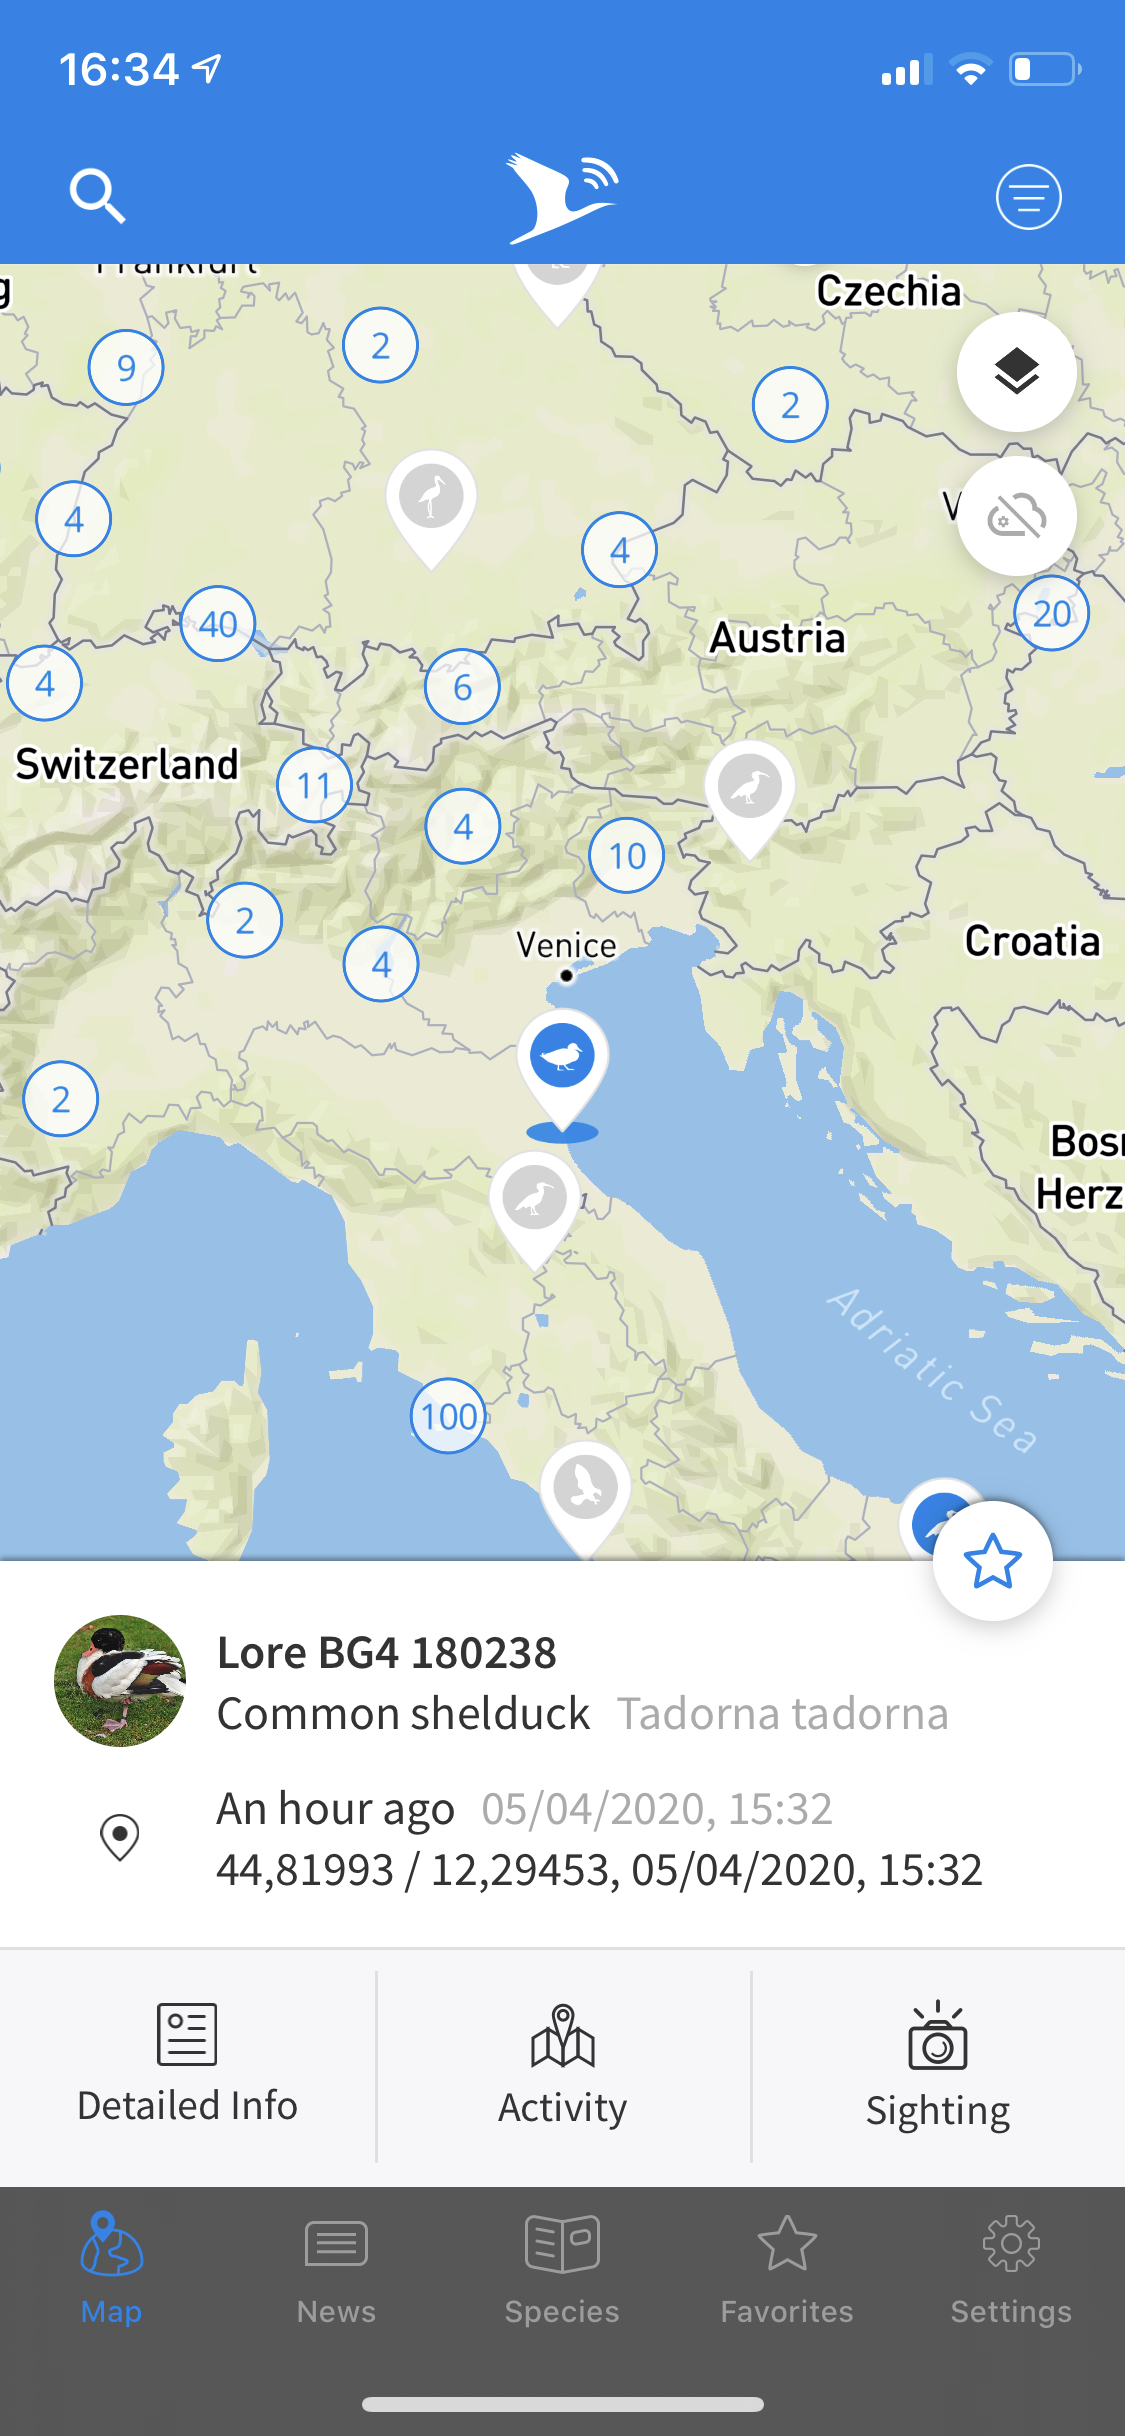
\includegraphics[width=70mm]{img/animaltracker_app_movebank.png}
	\end{center}
	\caption{Screenshot z aplikace Movebank Animal Tracker}
	\label{fig:movebank}
\end{figure}


\subsection{Anitra}

Anitra je českou ornitologickou značkou zabývající se vývojem a produkcí vlastních GPS-GSM trackovacích zařízení a poskytování softwarové platformy pro zobrazení dat a správu projektů. Rozdílem oproti platformám jiných výrobců je od základu jiná koncepce platformy. Platforma poskytovaná firmou Anitra průběžně integruje data z GPS-GSM trackerů od více výrobců a umožňuje nad daty dělat analýzy, automaticky je zpracovat dle předem stanovených pravidel, spravovat informace o jedincích, zadávat do aplikace vlastní body a přílohy. Od předem zmiňovaného Movebanku se aplikace liší především v možnosti ochranně vlastnictví dat, v aplikaci Anitra není povinnost data kdykoliv publikovat a majiteli dat zůstávají uživatelé. Aplikace taktéž umožňuje generovat uživatelsky přívětivé výstupy pro veřejnost či filtrovaná nebo plná data jednoduše sdílet mezi uživateli. Za podstatnou nevýhodu a nutnost využívat alternativní způsob zápisu v poli je především fakt, že platforma Anirta je řešena jako webová aplikace. V mobilních zařízeních je tedy obtížněji použitelná, ale hlavní nevýhodou je nutnost být stále připojen k internetu.

\begin{table}[h]
	\begin{tabular}{ | l | l | }
		\hline			
		Kritérium                              & Hodnocení \\
		\hline			
		Informace o jedincích                  & 1 -- detailní schéma vhodné pro ukládání informací o zvířatech          \\
		Práce s pozicemi z trackerů            & 1 -- aplikace přímo optimalizovaná pro tyto účely          \\
		Práce s uživatelsky vloženými pozicemi & 1 -- modul aplikace věnovaný pro vytváření těchto objektů          \\
		Přehlednost dat                        & 1 -- data lze zobrazit v mapě, tabulce, vyexportovat          \\
		Přenositelnost a sdílení dat           & 1 -- vlastník může vždy data vhodně vyexportovat          \\
		\hline	
	\end{tabular}
	\caption{Hodnocení Movebank}
\end{table}

\textbf{Výhody}

\begin{itemize}
	\item doménová specializace,
	\item dynamický rozvoj aplikace,
	\item 
\end{itemize}

\textbf{Nevýhody}

\begin{itemize}
	\item webová aplikace není vhodná pro použití v terénu,
	\item platforma není mezi ornitology příliš rozšířená,
	\item proprietární a nezdokumentované API.
\end{itemize}

